\begin{multicols}{3}[\section{Bluetooth Low Energy}]

\rhead{Autor: Sven Guthe}
\lfoot{Letzte Bearbeitung: 16.04.2016}

\newrefsegment

\begin{boxedminipage}{\linewidth}
\begin{tabular}{p{2,1 cm}p{2.7 cm}}
\textbf{Steckbrief}& \\
\end{tabular}
\begin{tabular}{p{2,1 cm}|p{2.7 cm}}
      Einsatz seit & Dezember 2009\\
      \hline
      Frequenz"-bereich  & \SI{2,4}{\giga\hertz}-Band mit 40 Kanälen zwischen \SI{2,402}{\giga\hertz} und \SI{2,483}{\giga\hertz}\\
      \hline
      Datenrate & \SI{0,27}{Mbit/s}\\
      \hline
      Verbreitung & Weltweit (vor allem Smart Wearables)\\
      \hline
      Reichweite & \SI{10}{\metre}\\
\end{tabular}
\end{boxedminipage}
\par

\subsection*{Überblick}
Bluetooth Low Energy (BLE) ist eine Kabellose Übertragungstechnologie, welche für Datenübertragungen zwischen kurzen Entfernungen von der Bluetooth Special Interest (SIG) Group entwickelt wurde. Wie die Bezeichnung der Technologie preisgibt, handelt es sich um eine Bluetooth-Spezifikation, bei welcher der energiesparsame Betrieb im Vordergrund steht um Verbindungen zu Geräten mit kleinem Energiespeicher herzustellen. Mit dieser Entwicklung, sichert sich der Bluetooth-Standard Anteile vor allem in den aufstrebenden Märkten der Gesundheitsindustrie (Fitnesstracker) und der Unterhaltungselektronik (Kopfhörer).
Zur Anwendung kommt BLE in Wearables wie Smartwatches, in Notebooks, in Smartphones und in vielen weiteren Geräten~\cite{BLE.4}.

\begin{Figure}
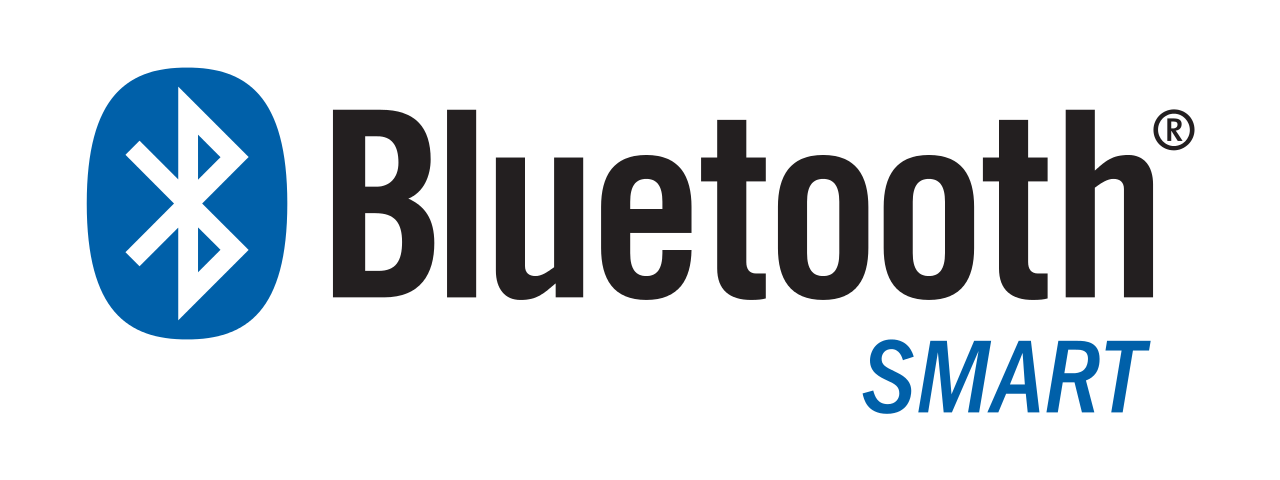
\includegraphics[width=\linewidth]{Kapitel/BLE/Grafiken/Bluetooth_Smart_Logo.png}
\captionof{figure}{Bluetooth Smart Logo~\cite{BLE.2}}
\end{Figure}

\subsection*{Technische Erläuterungen}
Eine Bluetooth Verbindung basiert auf einer Kommunikation zwischen einem Master und einem Slave. Der Master ist dabei das Gerät, welches die Verbindung initiiert. Dieser stellt auf 40 Kanälen eine Verbindung zum Slave her und kann dank des Frequenzsprungverfahren auf allen Kanälen parallel Daten senden, wodurch die Bandbreite enorm erhöht wird. Als Konsequenz ergibt sich aber, dass der Master-Takt bei allen verbundenen Slaves synchronisiert werden muss.
Eine Verbindung des Masters zu mehreren Slaves (max. 7) wird als "Piconet" bezeichnet. Befindet sich ein Gerät in mehreren Piconets, wird dies "Skatternet" genannt. Bei diesen Netzen kommt es zusätzlich noch zur Abstimmung der jeweiligen Sendekanäle und der Reihenfolge, in welcher die Daten in das jeweilige Netz gesendet werden.

Wie auch bei der Datenübertragung per WLAN werden die zu übersendenden Daten in Pakete unterteilt und versendet. Dabei wird bei dem Bluetooth Standard unterschieden zwischen einer synchronen (SCO - Synchronous Connection Oriented) und in einer asynchronen (ACL - Asynchronous ConnectionLess) Übertragung. Für die BLE-Technologie ist dabei vor allem die asynchrone Übertragung von Interesse. Dabei werden Daten zu einem beliebigen Zeitpunkt über die Pico-Netzwerke versendet und können gegebenenfalls erneut angefordert werden.

Ein Asynchrones Paket bestehet aus einer Identifikationssequenz (68-72 Bit, Access Code) zur Identifikation für das aktuelle Piconet, aus der Adresse des Slaves (3 Bit, Logical Transfer Address), einer Information über den verwendeten Pakettyp (4 Bit, Packet Type), 3 Flags, welche für das Blockieren des Controllers (Flow), für die Information, ob das letzte Paket erfolgreich angekommen ist (Automatic Repeat Request Number) und einer Sequenznummer (SEQN), um zu überprüfen, ob die Reihenfolge eingehalten wurde. Außerdem wird ein Hashwert (8 Bit, Header Error Check) angefügt, um ein mögliches falsches Paket zu erkennen. Hinter dieser festgesetzten Folge von Bits folgen schließlich die eigentlichen Informationen (0-2744 Bits, wobei nochmals 32 Bits für konkrete Informationen zum Paket verloren gehen)~\cite{BLE.1}.

\begin{Figure}
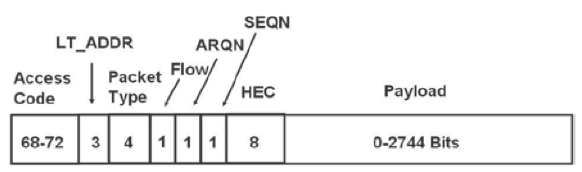
\includegraphics[width=\linewidth]{Kapitel/BLE/Grafiken/paket.png}
\captionof{figure}{ACL Paket~\cite{BLE.1}}
\end{Figure}

Übertragen werden die Informationen auf Frequenzen zwischen 2,402 GHz und 2,483 GHz auf 40 Kanälen. Damit kommt es zwar zwischen BLE und anderen Funktechnologie zu Überlagerungen, allerdings wechselt BLE seinen Sendekanal bis zu 1600 mal pro Sekunde.
Um die Übertragung entsprechend zu modulieren, wird der GFSK (Gaussian Frequency Shift Keying) Standard eingesetzt, bei der die schnell und stark ansteigenden Flanken abgeflacht und somit die für die Übertragung weniger Bandbreite benötigt wird.

Für die Übertragung werden Protokolle verwendet, welche denen aus dem bekannten OSI-Modell entsprechen. Dabei kommen die Schichten des Physical Layers in Form des Radio Layers und der Data Link Layer in Form des Baseband und des Link Manager Layers zum Einsatz. 
Der Radio Layer moduliert und demoduliert das Signal sowie versendet bzw. empfängt physikalische Signale. Der Baseband Layer sorgt für die Kontrolle der angekommenen Daten und sendet, falls nötig, eine Aufforderungen zur erneuten Sendung von fehlgeschlagenen Paketen aus. Zuletzt analysiert und verwaltet der Link Manager alle Verbindungen und setzt eine Authentifizierung zwischen Master und Slave sowie eine Verschlüsselung um.

Bei der Authentifizierung lässt BLE die Möglichkeiten offen, ob diese stattfinden muss oder nicht. Mithilfe des Object Push Profile (OPP) können Daten gesendet werden ohne jegliche Authentifizierung. Am Slave-Gerät muss nur bestätigt werden die Daten anzunehmen. Allerdings entspricht dies nicht dem Normalfall.
Wie bei dem Serial Port Profile müssen sich Geräte vor einer Datenübertragung pairen. Dazu ist es notwendig, einen zuvor ausgehandelten PIN einzugeben. Nach erfolgreichem Pairing, wird das verbundene Gerät in einer Liste von bekannten Geräten angezeigt. Neben dem Einsatz von PINs, wird auch das Pairing per NFC (Near Field Communication) immer mehr zum Standard.

Das Spezielle an dem Bluetooth Low Energy Standard sind die Zeitintervalle und die Datenmenge welche an gekoppelte Geräte übertragen werden. Anders als bei allen anderen Bluetooth Standards ist, dass BLE auf den Geräten nicht dauerhaft eingeschalten ist, sondern nur in gewissen Zeitabständen relevante Informationen sendet. Außerdem ist auch die Datenübertragung in ihrem Umfang eingeschränkt. Es werden maximal 220 kBit/s übertragen. Dies bedeutet, dass BLE nicht für alle Anwendungen in Frage kommt und bei größeren Datenmengen doch auf andere Standards zurückgegriffen werden muss. Durch den Fokus auf den stromsparenden Verbrauch von Bluetooth, wird neben der Datenrate und den Zeitabständen auch die Reichweite stark eingeschränkt. Von rund 100 Metern bei "normalen" Bluetooth sind bei BLE lediglich 10 Meter zu erreichen~\cite{BLE.1}.

\subsection*{Einsatz}
Die Einsatzmöglichkeiten von BLE sind sehr breitgefächert. Dabei wird auf einzelne Anwendungsgebiete genauer eingegangen. Ein durchaus gewinnbringender Einsatz ist im Einzelhandel möglich. Dabei können Geräte des Kunden im Geschäft automatisch Kontakt zu einem Bluetooth Access Point aufnehmen und Informationen über den Kunden und dessen Kaufverhalten an die Verkäufer senden. Interessanten Informationen wären dabei Browserverläufe, bei denen sich der Kunde auf der Suche nach Mode befand, vorausgesetzt der Kunde befindet sich in einem Modegeschäft. Neben den Möglichkeiten, den Verkäufer mit relevanten Informationen zu versorgen, ist es natürlich ebenfalls möglich, dem vermeintlichen Käufer einen Überblick über den Laden zu geben und benötigte Kleidung zu lokalisieren.

Das aber vermutlich gewinnbringendste Gebiet für BLE ist die Gesundheitsbranche. Geräte zum Puls anzeigen, Schritte zu messen oder auch Sportaktivitäten aufzuzeichnen sind bereits überall in allen Preisklassen erhältlich. Aber die Branche wird noch viel weiter gehen. Warum sollten nicht auch detailliertere Informationen über den Zustand des Körpers ermittelt und an das Handy bzw. direkt ans zuständige Krankenhaus gesendet werden. Mit kleinen Sensoren, welche über BLE verfügen, wäre dies realisierbar und stellt auch für den Nutzer einen Mehrwert dar, da er sich jeder Zeit über den Zustand seines Körpers informieren kann.

Auch in der Industrie bei der Wartung von Maschinen ist ein Verwenden von Bluetooth von großem Vorteil. Damit wäre es möglich, Fehler unabhängig von der Maschine, mit einem einzelnen portablen Gerät (Handy) abzulesen. Dies würde die Unternehmen unabhängiger von teurer Software der Entwickler machen und könnten die Oberflächen, je nach Anwendungsbedarf, selbst modifizieren.

Wie schon durch die drei aufgelisteten Bei-

\end{multicols}

\section*{Historische Entwicklung}
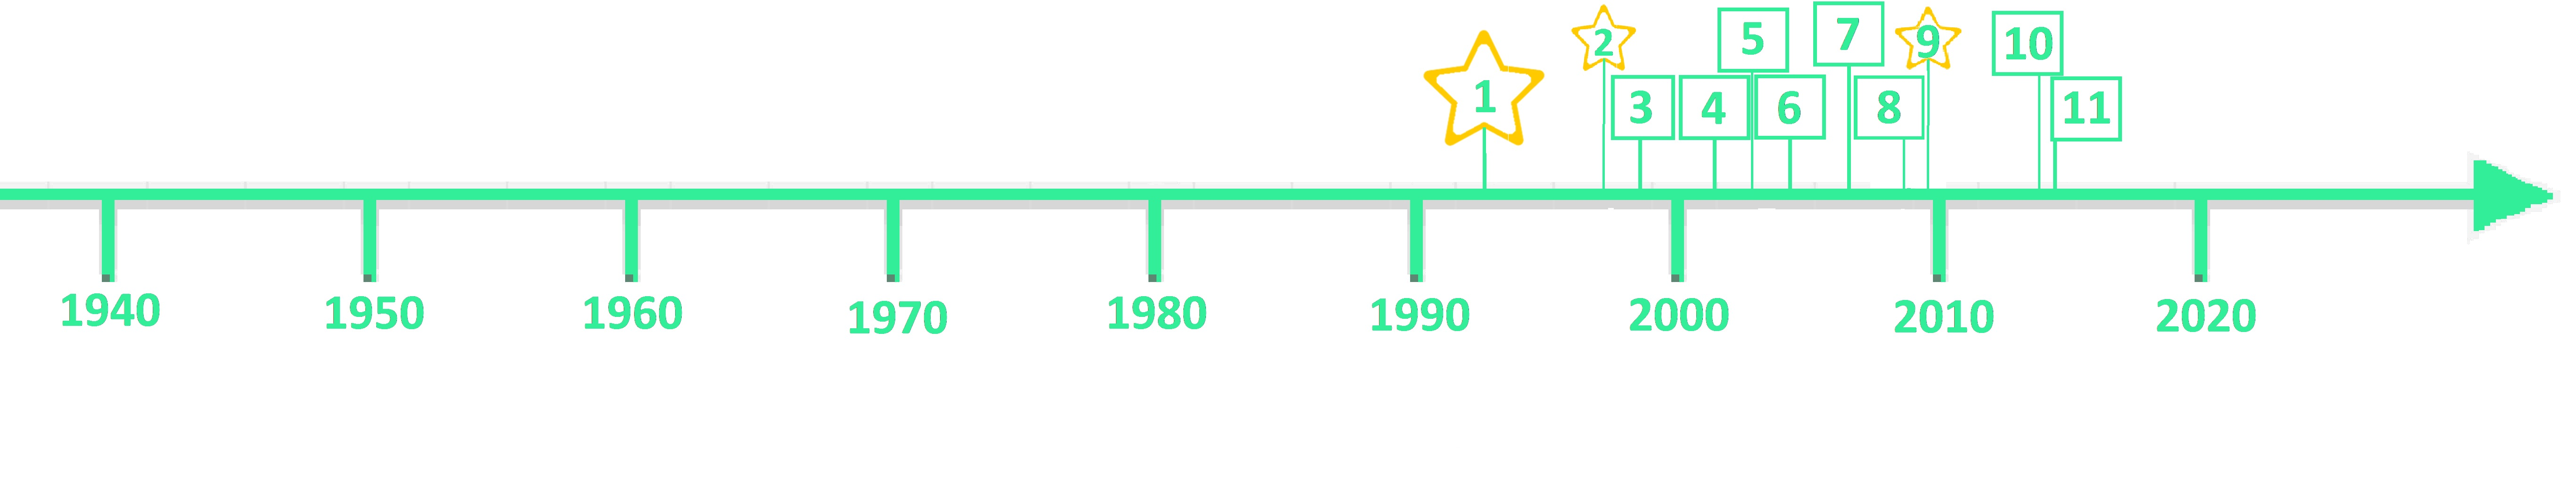
\includegraphics[width=\textwidth]{Kapitel/BLE/Grafiken/Zeitstrahl}
\par
\noindent
\begin{tabular}{|p{1 cm}|p{3 cm}|p{13.55 cm}|}
	\hline
	Nummer & Datum & Information \\
	\hline
	1 & August 1993 & Gründung der Infrared Data Association (IrDA) mit dem Ziel ein einheitliches Protokoll für Datenübertragung über Infrarot bereitzustellen.\\
	\hline
	2 & 1998 & Gründung der Bluetooth Special Interest Group (SIG) durch die Firmen Ericsson, Nokia, IBM, Toshiba und Intel zur Ausarbeitung eines Standards, der verbindliche Spezifikationen festlegte.\\
	\hline
	3 & Juli 1999 & Bereitstellung der Spezifikation Bluetooth 1.0 (Juli) und Bluetooth 1.0b (Dezember).\\
	\hline
	4 & Februar 2001 & Bereitstellung der Spezifikation Bluetooth 1.1.\\
	\hline
	5 & November 2003 & Bereitstellung der Spezifikation Bluetooth 1.2.\\
	\hline
	6 & November 2004 & Bereitstellung der Spezifikation Bluetooth 2.0 + EDR.\\
	\hline
	7 & August 2007 & Bereitstellung der Spezifikation Bluetooth 2.1 + EDR.\\
	\hline
	8 & April 2009 & Bereitstellung der Spezifikation Bluetooth 3.0 + HS.\\
	\hline
	\textbf{9} & \textbf{Dezember 2009} & \textbf{Bereitstellung der Spezifikation Bluetooth 4.0.}\\
	\hline
	10 & Dezember 2013 & Bereitstellung der Spezifikation Bluetooth 4.1.\\
	\hline
	11 & Dezember 2014 & Bereitstellung der Spezifikation Bluetooth 4.2.\\
	\hline
\end{tabular}
\par
\begin{multicols}{3}

spiele zu erkennen ist, ist Bluetooth in allen Gebieten des Lebens verwendbar in denen Daten übertragen werden müssen. Durch das Entwickeln des BLE Standards ist man zudem unabhängiger von Entwicklungen in der Batterieindustrie und kann mittels kleiner Energievorräte, Daten an kompatible Geräte senden. Damit wird BLE nicht nur für Konsumenten einen Mehrwert darstellen, sondern auch in der Entwicklung des "Internet der Dinge" (IoT - Internet of Things) in Verbindung mit SmartHome und anderen Technologien~\cite{BLE.1}.

\subsection*{Anbieter und Gremien}
Das Gremium, welches für die Entwicklung für neue Bluetooth Technologien zuständig ist, ist die schon genannte Bluetooth Special Interest (SIG) Group. Gegründet wurde dieses Gremium 1998 von den Unternehmen Nokia, Toshiba, Intel, IBM und Ericsson. Bis zum Jahre 1999 stiegen auch 3Com, Motorola, Lucent und Microsoft in die SIG Gruppe ein. SIG besitzt das Warenzeichen von Bluetooth und bestimmt mit den Entwicklungen der neuen Standards auch deren Spezifikationen. Mittlerweile wird das SIG Gremium von mehr als 30.000 Mitgliedern unterstützt~\cite{BLE.1}.

\begin{Figure}

\includegraphics[width=\linewidth]{Kapitel/BLE/Grafiken/BluetoothSIGLogo.jpg}
\captionof{figure}{Bluetooth SIG Logo~\cite{BLE.3}}
\end{Figure}

\subsection*{Ausblick}
Einen kleinen Ausblick konnte man schon bei den Einsatzgebieten einsehen, in denen man erkennen konnte, wie wichtig Bluetooth in der zukünftigen Vernetzung wird. Neben den Anwendungsgebieten, welche mit besseren Eigenschaften natürlich auch weiter steigen, sind auch neue Standards mit höheren Übertragungsraten auch im Low Energy Bereich geplant. Damit wird der BLE Standard auch für Anwendungen, in denen mehr Datenvolumen übertragen werden muss, interessant.

Das größte, interessanteste aber auch unberechenbarste Gebiet der Entwicklung für Übertragungstechnologie wird aber das "Internet der Dinge" darstellen. In der immer schnelleren Vernetzung des eigenen Zuhauses, des Körpers und andere Dinge des täglichen Lebens werden Übertragungsmöglichkeiten zwischen den Sensoren immer wichtiger. Ob sich der Bluetooth Standard dabei durchsetzt ist aufgrund der Schnelllebigkeit in Gebieten der Technik allerdings nicht zu beurteilen~\cite{BLE.1}.

\printbibliography[segment=4,heading=subbibliography]
\end{multicols}

\newpage
